\scanpage{6}
2/ Réciproquement, si $W$ est \deleted{ouvert et fermé}\inserted{stable par spécialisation}, alors $\pi^{-1}(W)\subset G\times W$ \deleted{est ouvert et fermé}\inserted{aussi}, donc stable par $G^0$, et contenant $e\times W$, il contient $G^0\times W$ \ldots. (Ici, on n'utilise pas l'hyp. sur les $\varphi$)

\figure{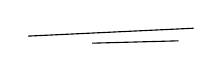
\begin{tikzpicture}\draw (0,0) -- (2.1,.10);\draw (.81,-.09) -- (1.91,-.06);\end{tikzpicture}}

\uline{Prop} Soit $G\xrightarrow{\deleted{\unsure{\lambda|v}}u}H$ \deleted{Si} hom de g.pes\deleted{, avec $G$ qu. cpt} Si $u$ est plat \inserted{(générisant)} en un p$^{\mathrm{t}}$, il est plat \deleted{(au \unsure{p. gén.})} \inserted{(\uline{univ} générisant)} \deleted{et \unsure{donc} \unsure{est} plat} ; \deleted{donc $u(G)$ stable par \deleted{spécialisation} générisat.}

% slanted
\margin{Il faut un argument pour ``univ'' générisant.}
\deleted{\uline{Cor} Supposons \deleted{que $H$ \unsure{qu cpt} qu'il existe} qu'il existe un p$^{\mathrm{t}}$ maximal $x$ de $H$ tel que $G_x\ne\varnothing$ (p. ex. $u$ dominant et $G$ qu. cpt) Alors \deleted{\unsure{$X$}} \inserted{si $H$ est réduit,} $u$ est plat, \deleted{donc généris\unsure{ant} (donc générisant \ldots)} Si on \inserted{ne} suppose pas \deleted{\uline{\unsure{Prop}} Su} avec $H$ réduit, $u$ est générisant, \deleted{et} l'image \deleted{\unsure{de}} $u(H)$ est stable \inserted{en} par générisation et \unsure{cont.|contient}}

\uline{Cor} Conditions équivalentes sur $u$

\deleted{\unsure{affine|ouvert}} a) $u$ est \inserted{univ} générisant \quad---\quad a$'$) $u$ générisant en un point.

b) $\unsure{U(G)|u(G)}\supset \deleted{G}H_0$

c) $\exists$ un point maximal \inserted{$x$} de $G$ tel que $u^{-1}(x)\ne\varnothing$.

Sous ces conditions, $u(G)$ est stable par spécialisation \deleted{(donc \unsure{fermé si} $G$ qu. cpt)}\margin{\deleted{\unsure{et H l. t. f.}}}

\uline{Dém} a) $\Longrightarrow$ a$'$) connu, a$'$) $\Longleftrightarrow$ b) \deleted{\illegible{1}} trivial, b) $\Longrightarrow$ c) trivial, prouvons c) $\longrightarrow$ b. Or $W=u(G)$ est stable \uline{par $\deleted{G}H_0$}, donc les $\varphi_x$ étant générisants, il est stable par spécialisation ; \deleted{OK} donc b) devient trivial.

% slanted
\margin{\deleted{avec} Est-il \uline{tjrs} vrai que $u(G)$ stable par spécialisation? Oui. Je prouve pour tt ss-ens. stable par mult (et sym.) $\to$ stable par spécia}
\uline{Cor} Si $G$ qu. cpt, \deleted{\unsure{domination} de $H^{\unsure{\mathrm{red}|\mathrm{t}}}$ \unsure{sur}} \inserted{$\operatorname{Im}u$ est fermée}

\uline{Prop.} Si $G\longrightarrow H$ un mono, avec $G$, \deleted{$H$} de t. f, \inserted{$H$ l. t. f.} alors $u$ est une immersion fermée.

\figure{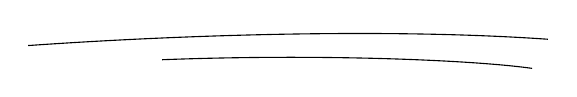
\begin{tikzpicture}\draw (0,0) .. controls (2,.14) and (4.6,.22) .. (6.6,.08);\draw (1.7,-.18) .. controls (3.8,-.10) and (5.7,-.19) .. (6.4,-.29);\end{tikzpicture}}

\diagram{$\displaystyle
\text{1)}\quad\left\{\begin{array}{l}
\text{Groupes discrets (ev. tordus)}\\
\text{Groupes profétales f. }(\text{---})\\
\text{Groupes loc. cpts (tot. discontinus) (ev. tordus}
\end{array}\right.
\quad\left|\begin{array}{l}
\text{groupes}\\
\text{séparables}\\
\text{tot. discontinus}
\end{array}\right.$}

\[
\begin{aligned}
\underline{\approx}\quad &\text{groupes topologiques loc. compact}\\
 &\text{\inserted{tot. disc.} avec opérations \uline{continues} de }\pi\\
 &\pi\times G\longrightarrow G\quad\text{continue.}
\end{aligned}
\]

\diagram{$\displaystyle
\text{2)}\quad\begin{array}{l|l}
\text{\uline{Groupes connexes}} & \text{\uline{sur corps parfait} : Extension (can.)}\\
\text{\uline{\deleted{\unsure{s|S}}Séparables}} & \text{d'une VA par un groupe connexe}\\
\text{[sont qu. cpts]} & \text{lisse affine}\quad\Longleftrightarrow\quad \underset{\longleftarrow}{\lim} G_i,\\
& \text{les }G_i\text{ de type fini, partie abélienne}\\
& \text{de dim. majorée.}
\end{array}$}
% archive sheet number: 5

